\documentclass{article}%
\usepackage[T1]{fontenc}%
\usepackage[utf8]{inputenc}%
\usepackage{lmodern}%
\usepackage{textcomp}%
\usepackage{lastpage}%
\usepackage[head=40pt,margin=0.5in,bottom=0.6in]{geometry}%
\usepackage{graphicx}%
%
\title{\textbf{Estudiante de la UCV resultó herida durante represión}}%
\author{El Nacional Web}%
\date{21/11/2018}%
%
\begin{document}%
\normalsize%
\maketitle%
\textbf{URL: }%
http://www.el{-}nacional.com/noticias/protestas/estudiante{-}ucv{-}resulto{-}herida{-}durante{-}represion\_260594\newline%
%
\textbf{Periodico: }%
EN, %
ID: %
260594, %
Seccion: %
Protestas\newline%
%
\textbf{Palabras Claves: }%
Estudiantes, Protestas, Sociedad\newline%
%
\textbf{Derecho: }%
1.3, %
Otros Derechos: %
, %
Sub Derechos: %
1.3.2.1\newline%
%
\textbf{EP: }%
SI\newline%
\newline%
%
\textbf{\textit{La joven se encontraba en la protesta que se registraba en la universidad}}%
\newline%
\newline%
%
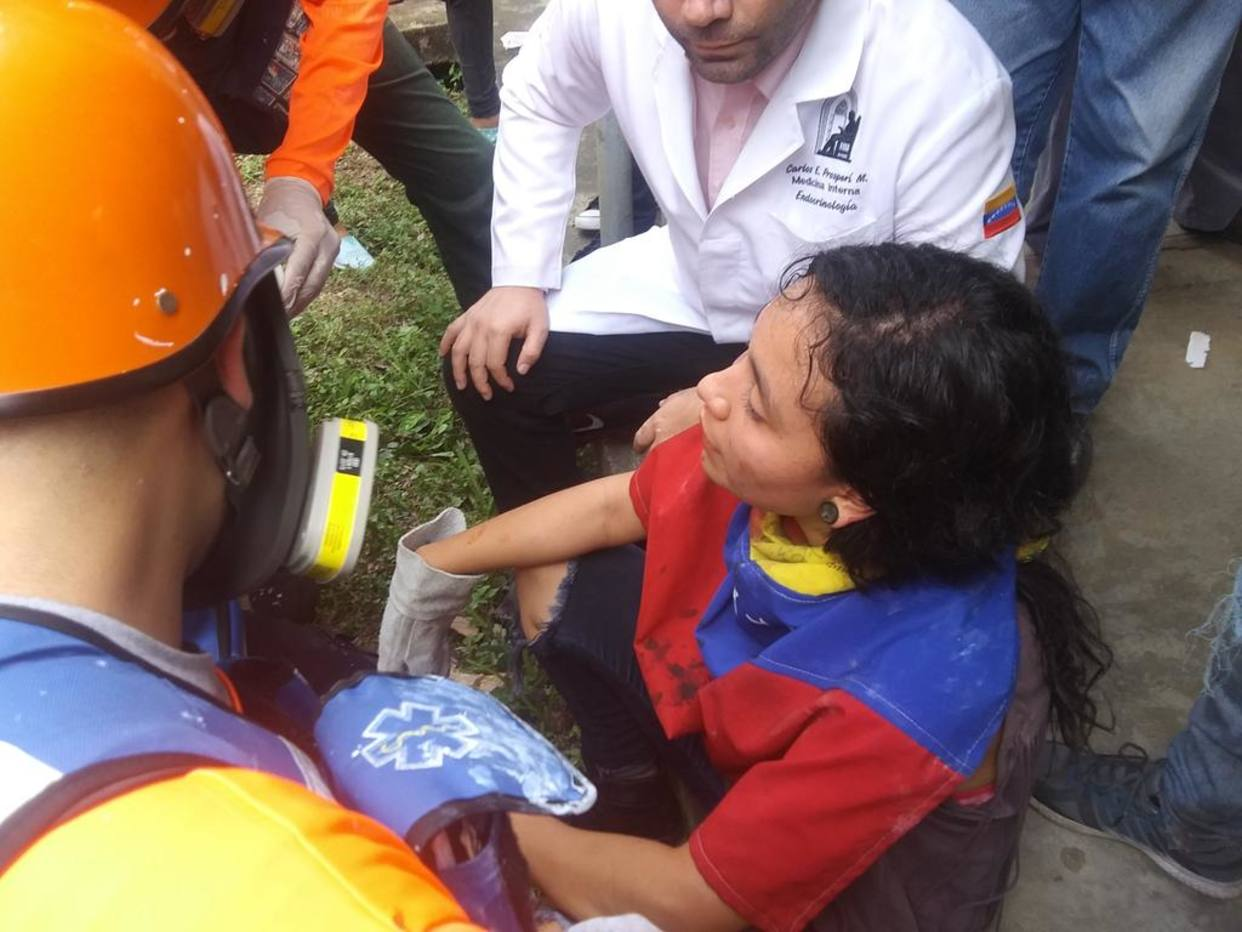
\includegraphics[width=300px]{70.jpg}%
\newline%
%
Una estudiante de la Universidad Central de Venezuela (UCV)~ resultó herida durante una protesta reprimida por~funcionarios de la Policía Nacional Bolivariana (PNB).%
\newline%
%
Los efectivos de la PNB~reprimieron la movilización de los estudiantes con gases lacrimógenos, los cuales afectaron~a las personas que se habían congregado.%
\newline%
%
De acuerdo con la información, la joven fue herida en la cara, específicamente en la mejilla~derecha~por la detonación de una bomba lacrimógena lanzada por un funcionario de la PNB.%
\newline%
%
Mediante videos difundidos en Twitter se observa a unos paramédicos atendiendo las heridas de los estudiantes.%
\newline%
%
Estudiantes de la UCV marcharon la mañana de este miércoles para conmemorar el Día del Estudiante Universitario. Además de denunciar la violación de la autonomía universitaria.%
\newline%
%
\end{document}